\documentclass[border=10pt]{standalone}
\usepackage{tikz}\usepackage{amsmath}\usetikzlibrary{arrows.meta,decorations.markings}
\begin{document}
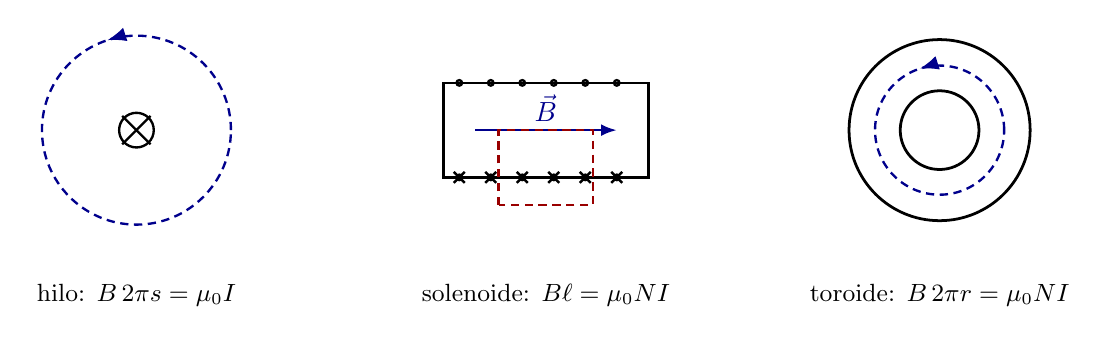
\begin{tikzpicture}[line width=0.85pt,>={Latex[length=2mm]}]
  % hilo + lazo circular
  \draw (-0.18,-0.18)--(0.18,0.18) (-0.18,0.18)--(0.18,-0.18);
  \draw (0,0) circle(0.22);
  \draw[blue!55!black,densely dashed,decoration={markings,mark=at position 0.3 with {\arrow{Latex}}},postaction={decorate}] (0,0) circle(1.2);
  \node at (0,-2.1){\small hilo: $B\,2\pi s=\mu_0 I$};
  % solenoide + lazo rectangular
  \begin{scope}[xshift=5.2cm]
    \draw[line width=1pt] (-1.3,0.6) rectangle (1.3,-0.6);
    \foreach \x in {-1.1,-0.7,...,1.3} {\draw (\x,0.6) circle(1pt);\fill (\x,0.6) circle(0.4pt);}
    \foreach \x in {-1.1,-0.7,...,1.3} {\draw (\x,-0.6) circle(1pt);\draw (\x-0.07,-0.67)--(\x+0.07,-0.53) (\x-0.07,-0.53)--(\x+0.07,-0.67);}
    \draw[->,blue!55!black] (-0.9,0)--(0.9,0); \node[blue!55!black] at (0,0.28){$\vec B$};
    \draw[red!60!black,densely dashed] (-0.6,-0.95) rectangle (0.6,0.0);
    \node at (0,-2.1){\small solenoide: $B\ell=\mu_0 N I$};
  \end{scope}
  % toroide
  \begin{scope}[xshift=10.2cm]
    \draw[line width=1pt] (0,0) circle(1.15);
    \draw[line width=1pt] (0,0) circle(0.5);
    \draw[blue!55!black,densely dashed,decoration={markings,mark=at position 0.3 with {\arrow{Latex}}},postaction={decorate}] (0,0) circle(0.82);
    \node at (0,-2.1){\small toroide: $B\,2\pi r=\mu_0 N I$};
  \end{scope}
\end{tikzpicture}
\end{document}
